%Quadcopter controller. Maybe not for masters but hobby 
%http://folk.ntnu.no/skoge/prost/proceedings/ecc-2013/data/papers/0927.pdf
%https://brage.bibsys.no/xmlui/bitstream/handle/11250/260353/435939_FULLTEXT01.pdf?sequence=3&isAllowed=y Model/methods
%https://ntrs.nasa.gov/archive/nasa/casi.ntrs.nasa.gov/20020060647.pdf



\subsection{Architectures}
    When integrating GNSS and INS data, the concept of \textit{coupledness} is important to consider. How coupled an integration architecture is describes its complexity with respect to which measurements are used \cite{groves2013principles, noureldin2012fundamentals}. Although different terms are found in the literature, the most widely used are \textit{loosely coupled}, \textit{tightly coupled} and \textit{deep integration}, as described in \cite{groves2013principles}. The integration filter output does not necessarily represent the actual state. In the indirect, or error state, filter error estimates of the INS solution is output instead. Further, if these error estimates are applied directly to the INS state estimate, the integration filter is said to be \textit{open loop}. The alternative is to supply the corrections as input to the INS, and is known as a \textit{closed loop} system.
    
    \subsubsection{Loosely coupled}
    A loosely integrated system favors modularity and simplicity for GNSS/INS integration, as shown in figure \ref{fig:loosely_coupled}. In this scheme, GNSS state estimates are used as measurement inputs to the integration filter, along with either raw IMU measurements or an INS state estimate. \\
    
    \begin{figure}
        \centering
        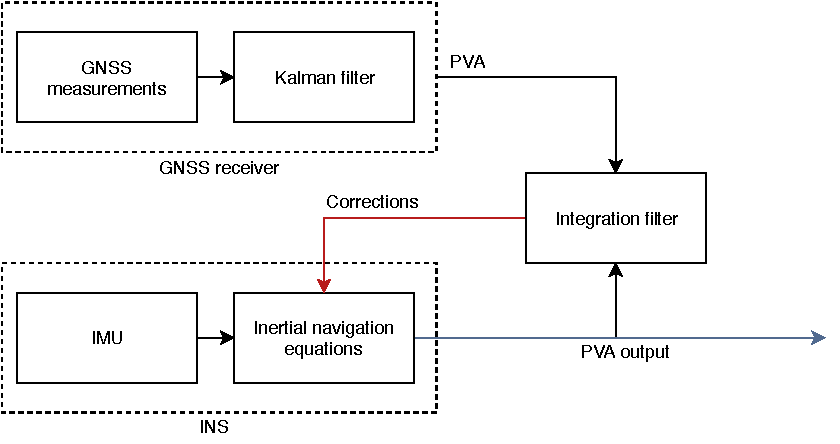
\includegraphics[scale=0.8]{Theory/bilder/loosely-coupled.pdf}
        \caption{A loosely coupled, closed loop system}
        \label{fig:loosely_coupled}
    \end{figure}
    
    The main drawback of this approach is that it tends to lead to cascaded Kalman filters. Because the estimates of a Kalman filter is based on propagation of earlier filter parameters, errors will be correlated in time. When the integration filter is implemented as a Kalman filter, it assumes that measurements are uncorrelated with respect to time, which is violated if the GNSS receiver implements a Kalman filter itself. This can significantly slow down the estimation of INS errors \cite{groves2013principles}. Another problems lies in the fact that the GNSS receiver will output no solution when the effective number of satellites fall below four. However, during normal operation the redundancy offered by the separate INS and GNSS solutions will maintain valid estimates even if the integration filter should fail.
    
    \subsubsection{Tightly coupled}
    %RTK: Tightly integrating INS with RTK measurements can result in a more robust system by decreasing the ambiguity resolution search space as aiding the detection of cycle slips \cite{li2017tightly}.
    The tightly integrated approach has no stand-alone GNSS solution, instead utilizing raw measurements from both an INS and a GNSS receiver in a single integration function. This approach does not suffer from the measurement bias introduced in a loosely coupled system, and the GNSS can still aid the INS even when fewer than four satellites are available. This approach tends to perform significantly better than the loosely coupled one, even when based on the same hardware \cite{falco2017loose, tawk2014implementation, groves2013principles}. \\

    \begin{figure}
        \centering
        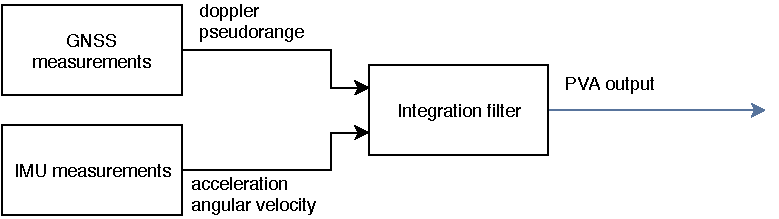
\includegraphics[scale=0.8]{Theory/bilder/tightly-coupled.pdf}
        \caption{A tightly coupled, direct integration filter}
        \label{fig:tightly_coupled}
    \end{figure}
    Figure \ref{fig:tightly_coupled} shows a tightly coupled integration architecture. Note that no Kalman filter is connected to the GNSS except for the integration filter, which utilizes the GNSS observables directly.\\

    \subsubsection{Deeply coupled}
    With access to a GNSS receivers firmware integration can be done \textit{ultra-tight}. This further couples the INS and GNSS receiver by using the INS to aid the receiver in signal tracking.
    
    
\subsection{Extended Kalman Filter}
%Estimates normal distribution, with the expected values representing the state and a covariance matrix that is propagated in step-wise, recursive computations.
    
The linear Kalman filter assumes that the error covariance follows a normal distribution. This assumption fails for non-linear systems. The Extended Kalman Filter solves this problem by applying linearized models to the covariance equations, while maintaining the nonlinear model for prediction and residual calculations. It should be noted that the extended case is not optimal, and the filter may diverge for inaccurate process models or poor initial state or error covariance estimates. \missingfigure[]{Confidence area (EKF)} %https://www.cbcity.de/das-extended-kalman-filter-einfach-erklaert\\

%Different noise modeleling can help. Model unconverged as extra large noise
%Confidence area should be an ellipsoid (The cause of the divergence of the Extended Kalman Filter is that, after some iterations, the actual state vector gets out of the ellipsoid that approximates the confidence area of the real state vector)
%https://www.ice.csic.es/files/perea/perea2006.pdf highly non-linear systems \\

    \subsubsection{Indirect implementation}
    Instead of having the filter estimate a state vector directly, it can be beneficial to integrate high frequency IMU measurements into a nominal state outside of the filter. This state vector is nominal in the sense that it ignores model imperfections and noise terms, which will eventually accumulate. Gaussian distributions of the accumulated errors can then be estimated in the Kalman filter, and their means injected into the nominal state. If the error state can be estimated and injected reasonably fast compared to the system dynamics, it can be assumed that accumulated errors are small in each correction step. In other words, the error state will operate close to the origin. and second order terms can be neglected, leading to simpler models and calculations \cite{sola2017quaternion}.\\
        
    When estimating the attitude of a body that may experience any orientation, a globally non-singular representation should be used for the nominal state. However, as the error state is assumed to operate close to the origin, far from any singularities, a minimal representation can be applied. This is beneficial in the case of the quaternion, as the redundant representation leads to a rank-deficient covariance, due to the unit constraint \cite{markley2003attitude}. Another benefit of the indirect filter, is that all the large-signal dynamics are integrated in the nominal state and corrections can therefore be applied at a lower rate than predictions \cite{sola2017quaternion}. For GNSS/INS integration, this is usually the case, where GNSS observables, used for corrections, arrive at a much lower frequency than INS measurements.
    
    \subsubsection{Multiplicative Extended Kalman Filter}
    \todo{Add PVA to abbrev}
    \todo{MEKF not necessarily indirect}
    The MEKF is a special implementation of an indirect EKF, used for PVA estimation. Error estimates are injected into the state estimate through through addition for all estimates except attitude, as adding the attitude error to the attitude estimate violates the quaternion unit constraint. By creating an error quaternion and injecting through the quaternion product operator, the quaternion estimate will only deviate from the unit constraint as numerical errors grow.

\todo{Use table?}
%\cite{kruglov2017modified}
\subsection{Attitude parametrizations}
There are numerous ways of representing attitude, a few interesting options will be looked into. \todo{Add more here. Talk about vectorial presentations and so on}

    \paragraph{Rotation vector}
    Following from Euler's theorem, the rotation of a rigid body can be described as the rotation by an angle $\phi$ about some axis. 

    \paragraph{Euler angles}
    An alternative to the vector parametrization approach are the Euler angles. Instead of using a single axis, the euler angles describe rotation as three \textit{simple rotations}; Three consecutive rotations about the basis vectors of some coordinate system. 

    \paragraph{Quaternions} \todo{Rewrite}
    It has been proved that no three dimensional parametrization of rotation can be globally nonsingular \cite{stuelpnagel1964parametrization}. The unit quaternion has the lowest dimensionality required for a globally nonsingular parametrization \cite{markley2003attitude}, and is represented as a four dimensional vector. It is also numerically efficient as the rotation of any vector is achieved through linear matrix multiplication \todo{Cite appendix?}. \\
    
    The rotation matrix of a quaternion $ \boldsymbol{q} = \begin{bmatrix} \eta & \bm{\varepsilon}\\ \end{bmatrix}^T$ can be written as \cite{fossen2011handbook}
    \begin{equation}
        \label{eq:quatRotMat}
        R_{\eta,\bm{\varepsilon}} = \bm{I_{3x3}} + 2\eta\bm{S}(\bm{\varepsilon}) + 2\bm{S}^2(\bm{\varepsilon})
    \end{equation}

    Using the relationship $\bm{S}(-\bm{\varepsilon}) = -\bm{S(\bm{\varepsilon})}$, it is evident that quaternions over-parametrize the rotation, as both $\bm{q}$ and $\bm{-q}$ represent the same rotation matrix. For this reason, it is customary to set the restriction $\eta > 0$ \cite{markley2003attitude}.

    \paragraph{Gibbs vector}
    The Gibbs vector is a projection of the quaternion space defined as
    \begin{equation}
        \label{eq:gibbs}
        \bm{g} \equiv \frac{\bm{\varepsilon}}{\eta}
    \end{equation}
    This is again a 2-1 mapping, where the Gibbs vector maps $\bm{q}$ and $\bm{-q}$ to the same point. However, because of the quaternion overparametrization, the resulting mapping is 1-1 for all rotations in the Euclidean space E3. The Gibbs vector introduces a singularity for $\eta = 0$, tending to infinity around this point, corresponding to a rotation of $180\degree$.

    \paragraph{Modified Rodrigues parameters}
    Fairly similar to the Gibbs vector, the modified Rodrigues parameters are defined as
    \begin{equation}
        \label{eq:modRodrigues}
        \bm{p} \equiv \frac{\bm{\varepsilon}}{\eta + 1}
    \end{equation}





%Structure
    % 1 - Motivation
    %     + Improving state estimation
    % 2 - Architectures
    %     + Loose
    %     + Tight
    %     + Ultra tight
    %     + Feedback vs open loop
    % 3 - Kalman filter
    %     + KF / EKF
    %       - Indirect implementation
    %           - Orientations state minimal. No over-parametrization
    %           - Operating close to the origin. Far away from singularities
    %           - Always small. Second-order products negligible
    %           - Error dynamics are small. All large dynamics already in nominal state. Can apply
    %           - corrections at a lower rate than predictions 
    %           - \cite{sola2017quaternion}
    %       - MEKF
    %           - Maintains quaternion unit length
    %     + Nonlinear observer(?)
    % 4 - Parametrizations
    %     + Vector-angle
    %     + Euler
    %     + Quaternion (Linear diff. eq. No EKF divergence)
    %     + Gibbs
    %     + Modified Rodrigues

%% Notes and keywords
% x The state variables in the KF is assumed to follow a normal distribution. 
% - Errors not assumed to be taken from normal dist. but yields exact joint prob. if so
% - No need to include earth rotation or bias rates if the resolution of the IMU is less than 10^-3 or so. (Assumed to be noise)
% - Tune Q and R by autocovariance least squares
% - Markov assumption: Initial state and noise vectors are mutually independent.
% - The Joseph form guarantees P to remain symmetric
% - Quaternions: 4 dim representation with 3 dof -> P singular or rank deficient. Euler angles has singularities. Avoid using trigonometric functions
% - Global vs local frame,